\section{A complete reproducible workflow, from a species list to a phylogeny, and distribution map.} 

If you aren't familiar with a complete workflow in R, it may be difficult to visualize the process. In R, everything is programmatic, so the whole workflow can be in one place, and be repeated whenever necessary. The following is a workflow for taxize, going from a species list to a phylogeny. 

First, install taxize

\begin{knitrout}
\definecolor{shadecolor}{rgb}{0.969, 0.969, 0.969}\color{fgcolor}\begin{kframe}
\begin{alltt}
\hlfunctioncall{install.packages}(\hlstring{"taxize"})
\end{alltt}
\end{kframe}
\end{knitrout}


Then load it into R

\begin{knitrout}
\definecolor{shadecolor}{rgb}{0.969, 0.969, 0.969}\color{fgcolor}\begin{kframe}
\begin{alltt}
\hlfunctioncall{library}(taxize)
\end{alltt}
\end{kframe}
\end{knitrout}


Most of us will start out with a species list, something like the one below. Note that each of the names is spelled incorrectly.

\begin{knitrout}
\definecolor{shadecolor}{rgb}{0.969, 0.969, 0.969}\color{fgcolor}\begin{kframe}
\begin{alltt}
splist <- \hlfunctioncall{c}(\hlstring{"Helanthus annuus"}, \hlstring{"Pinos contorta"}, \hlstring{"Collomia grandiflorra"}, \hlstring{"Abies magnificaa"}, 
    \hlstring{"Rosa california"}, \hlstring{"Datura wrighti"}, \hlstring{"Mimulus bicolour"}, \hlstring{"Nicotiana glauca"}, 
    \hlstring{"Maddia sativa"}, \hlstring{"Bartlettia scapposa"})
\end{alltt}
\end{kframe}
\end{knitrout}


There are many ways to resolve taxonomic names in taxize. Of course, the ideal name resolver will do the work behind the scenes for you so that you don't have to do things like fuzzy matching. There are a few services in taxize like this we can choose from: the Global Names Resolver service from EOL (see function \emph{gnr\_resolve}) and the Taxonomic Name Resolution Service from iPlant (see function \emph{tnrs}). In this case let's use the function \emph{tnrs}. 

\begin{knitrout}
\definecolor{shadecolor}{rgb}{0.969, 0.969, 0.969}\color{fgcolor}\begin{kframe}
\begin{alltt}
\hlcomment{# The tnrs function accepts a vector of 1 or more}
splist_tnrs <- \hlfunctioncall{tnrs}(query = splist, getpost = \hlstring{"POST"}, source_ = \hlstring{"iPlant_TNRS"})
\end{alltt}


{\ttfamily\noindent\itshape\color{messagecolor}{\#\# Calling http://taxosaurus.org/retrieve/679c69546d1311b72ce97f5ad1101254}}\begin{alltt}

\hlcomment{# Remove some fields}
(splist_tnrs <- splist_tnrs[, !\hlfunctioncall{names}(splist_tnrs) %in% \hlfunctioncall{c}(\hlstring{"matchedName"}, \hlstring{"annotations"}, 
    \hlstring{"uri"})])
\end{alltt}
\begin{verbatim}
##            submittedName         acceptedName    sourceId score
## 3       Helanthus annuus    Helianthus annuus iPlant_TNRS  0.98
## 1         Pinos contorta       Pinus contorta iPlant_TNRS  0.96
## 4  Collomia grandiflorra Collomia grandiflora iPlant_TNRS  0.99
## 5       Abies magnificaa      Abies magnifica iPlant_TNRS  0.98
## 10       Rosa california     Rosa californica iPlant_TNRS  0.99
## 9         Datura wrighti      Datura wrightii iPlant_TNRS  0.98
## 7       Mimulus bicolour      Mimulus bicolor iPlant_TNRS  0.98
## 8       Nicotiana glauca     Nicotiana glauca iPlant_TNRS  1.00
## 6          Maddia sativa         Madia sativa iPlant_TNRS  0.97
## 2    Bartlettia scapposa   Bartlettia scaposa iPlant_TNRS  0.98
\end{verbatim}
\begin{alltt}

\hlcomment{# Note the scores. They suggest that there were no perfect matches, but}
\hlcomment{# they were all very close, ranging from 0.77 to 0.99 (1 is the highest).}
\hlcomment{# Let's assume the names in the 'acceptedName' column are correct (and}
\hlcomment{# they should be).}

\hlcomment{# So here's our updated species list}
(splist <- \hlfunctioncall{as.character}(splist_tnrs$acceptedName))
\end{alltt}
\begin{verbatim}
##  [1] "Helianthus annuus"    "Pinus contorta"       "Collomia grandiflora"
##  [4] "Abies magnifica"      "Rosa californica"     "Datura wrightii"     
##  [7] "Mimulus bicolor"      "Nicotiana glauca"     "Madia sativa"        
## [10] "Bartlettia scaposa"
\end{verbatim}
\end{kframe}
\end{knitrout}


Another thing we may want to do is collect common names for our taxa. 

\begin{knitrout}
\definecolor{shadecolor}{rgb}{0.969, 0.969, 0.969}\color{fgcolor}\begin{kframe}
\begin{alltt}
tsns <- \hlfunctioncall{get_tsn}(searchterm = splist, searchtype = \hlstring{"sciname"}, verbose = FALSE)
comnames <- \hlfunctioncall{lapply}(tsns, getcommonnamesfromtsn)
\end{alltt}


{\ttfamily\noindent\itshape\color{messagecolor}{\#\# http://www.itis.gov/ITISWebService/services/ITISService/getCommonNamesFromTSN?tsn=36616}}

{\ttfamily\noindent\itshape\color{messagecolor}{\#\# http://www.itis.gov/ITISWebService/services/ITISService/getCommonNamesFromTSN?tsn=183327}}

{\ttfamily\noindent\itshape\color{messagecolor}{\#\# http://www.itis.gov/ITISWebService/services/ITISService/getCommonNamesFromTSN?tsn=31037}}

{\ttfamily\noindent\itshape\color{messagecolor}{\#\# http://www.itis.gov/ITISWebService/services/ITISService/getCommonNamesFromTSN?tsn=181834}}

{\ttfamily\noindent\itshape\color{messagecolor}{\#\# http://www.itis.gov/ITISWebService/services/ITISService/getCommonNamesFromTSN?tsn=24818}}

{\ttfamily\noindent\itshape\color{messagecolor}{\#\# http://www.itis.gov/ITISWebService/services/ITISService/getCommonNamesFromTSN?tsn=30521}}

{\ttfamily\noindent\itshape\color{messagecolor}{\#\# http://www.itis.gov/ITISWebService/services/ITISService/getCommonNamesFromTSN?tsn=33245}}

{\ttfamily\noindent\itshape\color{messagecolor}{\#\# http://www.itis.gov/ITISWebService/services/ITISService/getCommonNamesFromTSN?tsn=30574}}

{\ttfamily\noindent\itshape\color{messagecolor}{\#\# http://www.itis.gov/ITISWebService/services/ITISService/getCommonNamesFromTSN?tsn=38040}}

{\ttfamily\noindent\itshape\color{messagecolor}{\#\# http://www.itis.gov/ITISWebService/services/ITISService/getCommonNamesFromTSN?tsn=36822}}\begin{alltt}

\hlcomment{# Unfortunately, common names are not standardized like species names, so}
\hlcomment{# there are multiple common names for each taxon}
\hlfunctioncall{sapply}(comnames, length)
\end{alltt}
\begin{verbatim}
##  [1] 3 3 3 3 3 3 3 3 3 3
\end{verbatim}
\begin{alltt}

\hlcomment{# So let's just take the first common name for each species}
comnames_vec <- \hlfunctioncall{do.call}(c, \hlfunctioncall{lapply}(comnames, \hlfunctioncall{function}(x) \hlfunctioncall{as.character}(x[1, \hlstring{"comname"}])))

\hlcomment{# And we can make a data.frame of our scientific and common names}
(allnames <- \hlfunctioncall{data.frame}(spname = splist, comname = comnames_vec))
\end{alltt}
\begin{verbatim}
##                  spname                       comname
## 1     Helianthus annuus              common sunflower
## 2        Pinus contorta                lodgepole pine
## 3  Collomia grandiflora        largeflowered collomia
## 4       Abies magnifica                    golden fir
## 5      Rosa californica           California wildrose
## 6       Datura wrightii            sacred thorn-apple
## 7       Mimulus bicolor yellow and white monkeyflower
## 8      Nicotiana glauca                  tree tobacco
## 9          Madia sativa                 coast tarweed
## 10   Bartlettia scaposa                Bartlett daisy
\end{verbatim}
\end{kframe}
\end{knitrout}


Another common task is getting the taxonomic tree upstream from your study taxa. We often know what family or order our taxa are in, but it we often don't know the tribes, subclasses, and superfamilies. taxize provides many avenues to getting classifications. Two of them are accessible via a single function (\emph{classification}): the Integrated Taxonomic Information System (ITIS) and National Center for Biotechnology Information (NCBI); and via the Catalogue of Life (see function \emph{col\_classification}):

\begin{knitrout}
\definecolor{shadecolor}{rgb}{0.969, 0.969, 0.969}\color{fgcolor}\begin{kframe}
\begin{alltt}
\hlcomment{# As we already have Taxonomic Serial Numbers from ITIS, let's just get}
\hlcomment{# classifications from ITIS. Note that we could use uBio instead.}
class_list <- \hlfunctioncall{classification}(tsns)
\end{alltt}


{\ttfamily\noindent\itshape\color{messagecolor}{\#\# http://www.itis.gov/ITISWebService/services/ITISService/getFullHierarchyFromTSN?tsn=36616}}

{\ttfamily\noindent\itshape\color{messagecolor}{\#\# http://www.itis.gov/ITISWebService/services/ITISService/getFullHierarchyFromTSN?tsn=183327}}

{\ttfamily\noindent\itshape\color{messagecolor}{\#\# http://www.itis.gov/ITISWebService/services/ITISService/getFullHierarchyFromTSN?tsn=31037}}

{\ttfamily\noindent\itshape\color{messagecolor}{\#\# http://www.itis.gov/ITISWebService/services/ITISService/getFullHierarchyFromTSN?tsn=181834}}

{\ttfamily\noindent\itshape\color{messagecolor}{\#\# http://www.itis.gov/ITISWebService/services/ITISService/getFullHierarchyFromTSN?tsn=24818}}

{\ttfamily\noindent\itshape\color{messagecolor}{\#\# http://www.itis.gov/ITISWebService/services/ITISService/getFullHierarchyFromTSN?tsn=30521}}

{\ttfamily\noindent\itshape\color{messagecolor}{\#\# http://www.itis.gov/ITISWebService/services/ITISService/getFullHierarchyFromTSN?tsn=33245}}

{\ttfamily\noindent\itshape\color{messagecolor}{\#\# http://www.itis.gov/ITISWebService/services/ITISService/getFullHierarchyFromTSN?tsn=30574}}

{\ttfamily\noindent\itshape\color{messagecolor}{\#\# http://www.itis.gov/ITISWebService/services/ITISService/getFullHierarchyFromTSN?tsn=38040}}

{\ttfamily\noindent\itshape\color{messagecolor}{\#\# http://www.itis.gov/ITISWebService/services/ITISService/getFullHierarchyFromTSN?tsn=36822}}\begin{alltt}
\hlfunctioncall{sapply}(class_list, nrow)
\end{alltt}
\begin{verbatim}
##  [1] 12 11 12 11 12 12 12 12 12 12
\end{verbatim}
\begin{alltt}

\hlcomment{# And we can attach these names to our allnames data.frame}
\hlfunctioncall{library}(plyr)
gethiernames <- \hlfunctioncall{function}(x) \{
    temp <- x[, \hlfunctioncall{c}(\hlstring{"rankName"}, \hlstring{"taxonName"})]
    values <- \hlfunctioncall{data.frame}(\hlfunctioncall{t}(temp[, 2]))
    \hlfunctioncall{names}(values) <- temp[, 1]
    \hlfunctioncall{return}(values)
\}
class_df <- \hlfunctioncall{ldply}(class_list, gethiernames)
allnames_df <- \hlfunctioncall{merge}(allnames, class_df, by.x = \hlstring{"spname"}, by.y = \hlstring{"Species"})

\hlcomment{# Now that we have allnames_df, we can start to see some relationships}
\hlcomment{# among species simply by their shared taxonomic names}
allnames_df[1:2, ]
\end{alltt}
\begin{verbatim}
##               spname        comname Kingdom     Subkingdom Infrakingdom
## 1    Abies magnifica     golden fir Plantae Viridaeplantae Streptophyta
## 2 Bartlettia scaposa Bartlett daisy Plantae Viridaeplantae Streptophyta
##       Division     Subdivision Infradivision         Class Superorder
## 1 Tracheophyta Spermatophytina  Gymnospermae     Pinopsida       <NA>
## 2 Tracheophyta Spermatophytina  Angiospermae Magnoliopsida  Asteranae
##       Order     Family      Genus
## 1   Pinales   Pinaceae      Abies
## 2 Asterales Asteraceae Bartlettia
\end{verbatim}
\begin{alltt}

\hlcomment{# Ah, so Abies and Bartlettia are in different infradivisions, but share}
\hlcomment{# taxonomic names above that point.}
\end{alltt}
\end{kframe}
\end{knitrout}


However, taxonomy can only get you so far. Shared ancestry can be reconstructed from molecular data, and phylogenies created. Phylomatic is a web service with an API that we can use to get a phylogeny. 

\begin{figure}[!h] 
\centering 
\begin{knitrout}
\definecolor{shadecolor}{rgb}{0.969, 0.969, 0.969}\color{fgcolor}\begin{kframe}
\begin{alltt}
\hlcomment{# Fetch phylogeny from phylomatic}
phylogeny <- \hlfunctioncall{phylomatic_tree}(taxa = \hlfunctioncall{as.character}(allnames$spname), taxnames = TRUE, 
    get = \hlstring{"POST"}, informat = \hlstring{"newick"}, method = \hlstring{"phylomatic"}, storedtree = \hlstring{"R20120829"}, 
    taxaformat = \hlstring{"slashpath"}, outformat = \hlstring{"newick"}, clean = \hlstring{"true"}, parallel = TRUE)
\end{alltt}


{\ttfamily\noindent\color{warningcolor}{\#\# Warning: No parallel backend registered}}

{\ttfamily\noindent\color{warningcolor}{\#\# Warning: executing \%dopar\% sequentially: no parallel backend registered}}\begin{alltt}
\hlcomment{# Format teeth-labels}
phylogeny$tip.label <- \hlfunctioncall{capwords}(phylogeny$tip.label, onlyfirst = TRUE)
\hlcomment{# plot phylogeny}
\hlfunctioncall{plot}(phylogeny)
\end{alltt}
\end{kframe}
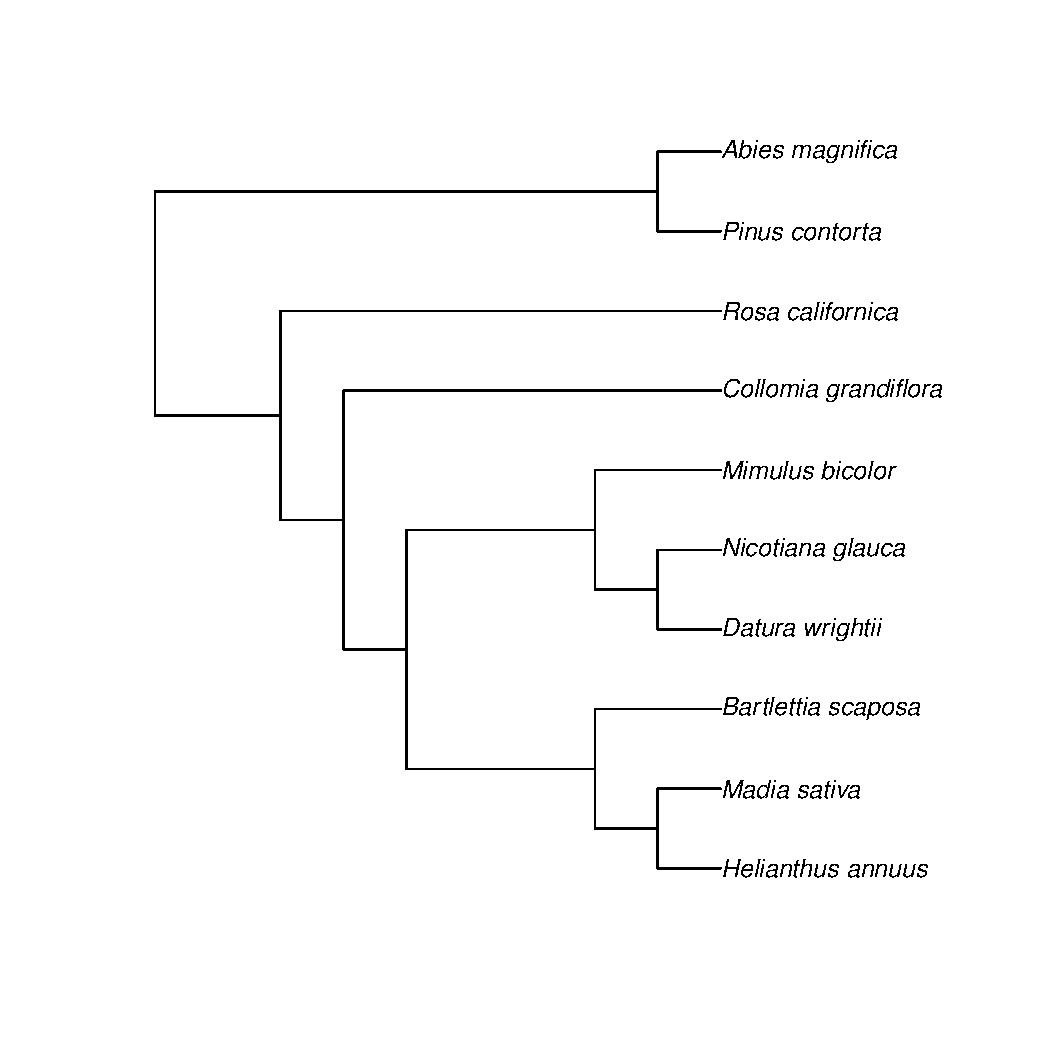
\includegraphics[width=4in,height=4in]{figure/phylogeny} 

\end{knitrout}

\caption{a phylogeny...} 
\end{figure} 

Using the species list, with the corrected names, we can now search for occurrence data. The Global Biodiversity Information Facility (GBIF) has the largest collection of records data, and has a  API that we can interact with programmatically from R. First, we need to install rgbif.

\begin{knitrout}
\definecolor{shadecolor}{rgb}{0.969, 0.969, 0.969}\color{fgcolor}\begin{kframe}
\begin{alltt}
\hlcomment{# Install rgbif from github.com}
\hlfunctioncall{install.packages}(\hlstring{"devtools"})
\hlfunctioncall{library}(devtools)
\hlfunctioncall{install_github}(\hlstring{"rgbif"}, \hlstring{"ropensci"})
\end{alltt}
\end{kframe}
\end{knitrout}


Now we can search for occurrences for our species list and make a map.


\begin{knitrout}
\definecolor{shadecolor}{rgb}{0.969, 0.969, 0.969}\color{fgcolor}\begin{kframe}
\begin{alltt}
\hlfunctioncall{library}(rgbif)
\hlfunctioncall{library}(ggplot2)

\hlcomment{# get occurences}
occurr_list <- \hlfunctioncall{occurrencelist_many}(\hlfunctioncall{as.character}(allnames$spname), coordinatestatus = TRUE, 
    maxresults = 100, removeZeros = TRUE, fixnames = \hlstring{"changealltorig"})
\end{alltt}


{\ttfamily\noindent\color{warningcolor}{\#\# Warning: NAs introduced by coercion}}

{\ttfamily\noindent\color{warningcolor}{\#\# Warning: NAs introduced by coercion}}

{\ttfamily\noindent\color{warningcolor}{\#\# Warning: NAs introduced by coercion}}

{\ttfamily\noindent\color{warningcolor}{\#\# Warning: NAs introduced by coercion}}

{\ttfamily\noindent\color{warningcolor}{\#\# Warning: NAs introduced by coercion}}

{\ttfamily\noindent\color{warningcolor}{\#\# Warning: NAs introduced by coercion}}

{\ttfamily\noindent\color{warningcolor}{\#\# Warning: NAs introduced by coercion}}

{\ttfamily\noindent\color{warningcolor}{\#\# Warning: NAs introduced by coercion}}

{\ttfamily\noindent\color{warningcolor}{\#\# Warning: NAs introduced by coercion}}

{\ttfamily\noindent\color{warningcolor}{\#\# Warning: NAs introduced by coercion}}

{\ttfamily\noindent\color{warningcolor}{\#\# Warning: NAs introduced by coercion}}

{\ttfamily\noindent\color{warningcolor}{\#\# Warning: NAs introduced by coercion}}

{\ttfamily\noindent\color{warningcolor}{\#\# Warning: NAs introduced by coercion}}

{\ttfamily\noindent\color{warningcolor}{\#\# Warning: NAs introduced by coercion}}

{\ttfamily\noindent\color{warningcolor}{\#\# Warning: NAs introduced by coercion}}

{\ttfamily\noindent\color{warningcolor}{\#\# Warning: NAs introduced by coercion}}\begin{alltt}

\hlcomment{# Make a map}
p <- \hlfunctioncall{gbifmap}(occurr_list) + \hlfunctioncall{guides}(col = \hlfunctioncall{guide_legend}(title = \hlstring{""}, nrow = 3, 
    byrow = TRUE)) + \hlfunctioncall{theme}(legend.position = \hlstring{"bottom"}, legend.key = \hlfunctioncall{element_blank}()) + 
    \hlfunctioncall{coord_equal}()
\end{alltt}


{\ttfamily\noindent\itshape\color{messagecolor}{\#\# Rendering map...plotting 623 points}}\begin{alltt}
p
\end{alltt}
\end{kframe}\begin{figure}[h]

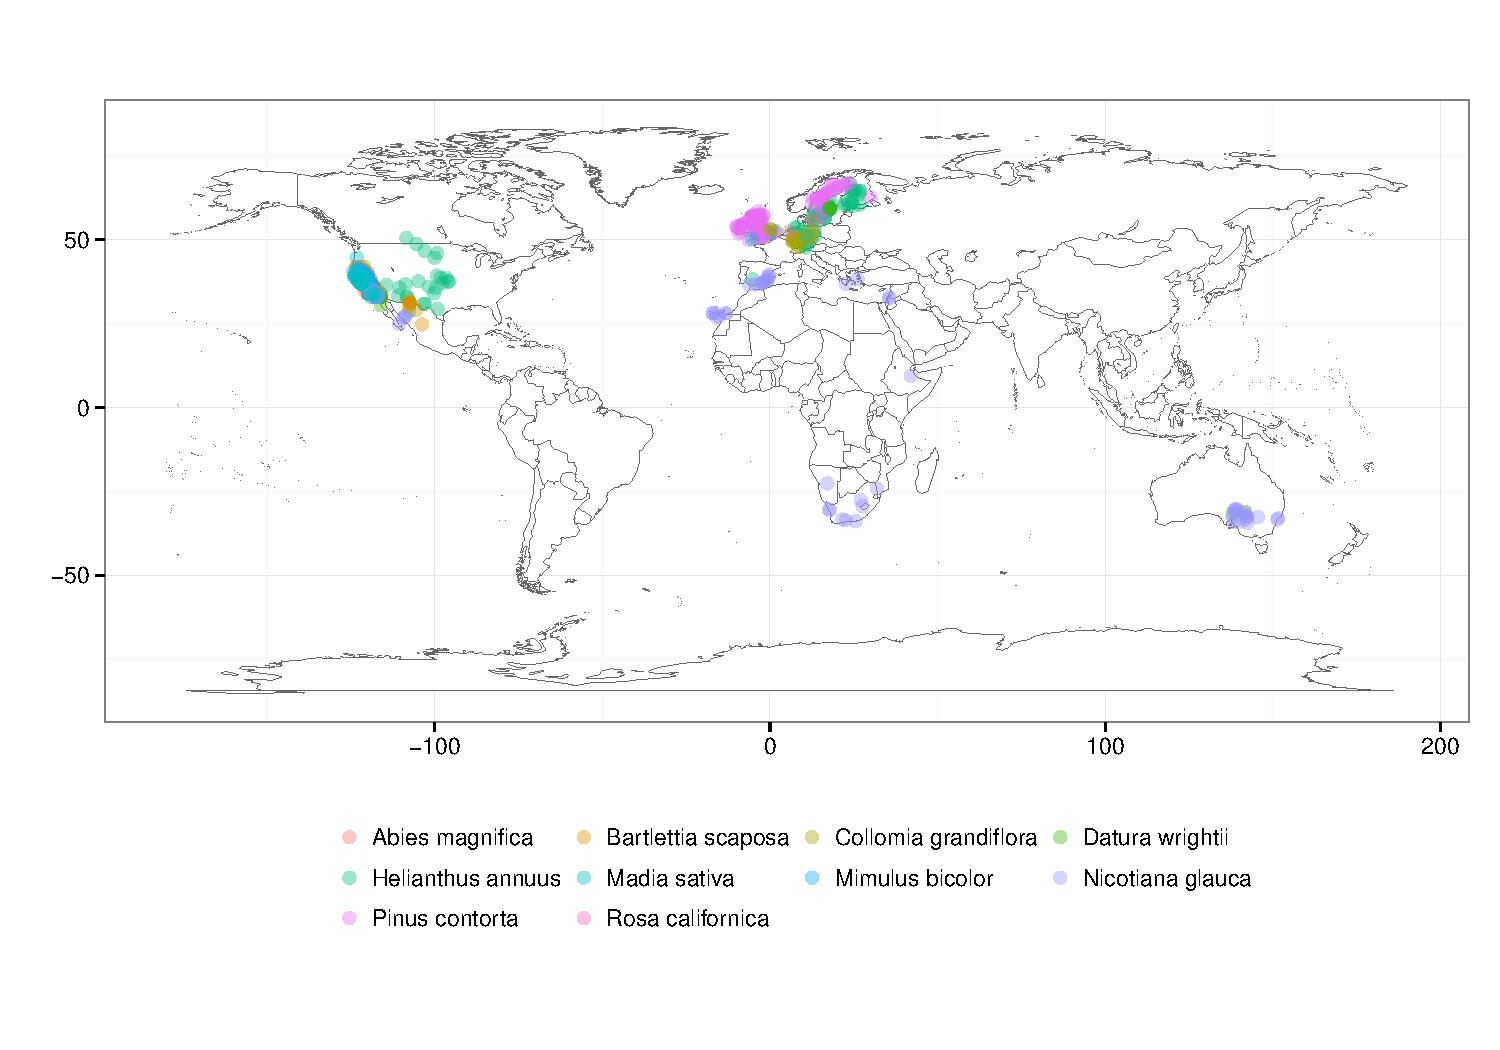
\includegraphics[width=.9\textwidth]{figure/plot_map} \caption[A map]{A map\label{fig:mapplot_map}}
\end{figure}


\end{knitrout}

